\documentclass[12pt,a4paper,twoside]{book}
\usepackage{graphicx}
\usepackage{setspace}	%double spacing for text, single for captions, footnotes, etc.
%\usepackage{hypernat} 	%substitut de cite que permet fer hyperlinks
\usepackage{natbib}		% substituye a 'hypernat' que funciona en Windows.
\usepackage[english]{babel}
\usepackage[utf8]{inputenc}
\usepackage{color}
\usepackage{hhline} 		% extended styles for tables
\usepackage{multirow}
\usepackage{subfigure}
\usepackage{acronym}
\usepackage{hyperref}
\usepackage{amsmath,amsmath,amssymb} 
\usepackage{fancyhdr}
\usepackage{epsfig, amsmath}
\usepackage{algorithm}
\usepackage{algorithmic}
\usepackage{epigraph}
\usepackage{csquotes}
\usepackage{float}

% general settings
\hypersetup{
	linktocpage=true,
	colorlinks=true,
	linkcolor=blue,
	citecolor=blue,
}
\definecolor{Hgray}{gray}{0.6}

\newenvironment{definition}[1][Definition]{\begin{trivlist}
\item[\hskip \labelsep {\bfseries #1}]}{\end{trivlist}}

\setlength{\topmargin}{0cm}
\setlength{\textheight}{23cm}
\setlength{\textwidth}{17cm}
\setlength{\oddsidemargin}{0cm}
\setlength{\evensidemargin}{0cm}
\setlength{\headheight}{1cm}

% indica que las 'sub-sub-sections' sean numeradas y aparezcan en el indice
\setcounter{secnumdepth}{3}
\setcounter{tocdepth}{2}

% settings for code
\renewcommand{\algorithmicrequire}{\textbf{Entrada: }}
\renewcommand{\algorithmicensure}{\textbf{Salida: }}

%%%%%%%%%%%%
% DOCUMENT %
%%%%%%%%%%%%
\begin{document}

% portada
\newpage
\thispagestyle{empty}

\baselineskip 2em

%\vspace*{1cm}

\centerline{
\includegraphics[width=0.6\textwidth]{images/UOC-logo}}
\begin{center}
\textsc{Universitat Oberta de Catalunya (UOC) \\
Data Science master's degree (\textit{Data Science})\\}

%\centerline {\pic{UOC}{4cm}}

\vspace*{1.5cm}

\textsc{\Large MASTER'S DEGREE FINAL WORK}

\vspace*{0.5cm}

\textsc{\large Area: 5}


%\textbf{\Huge VirtualTechLab Model: }

\vspace*{2.0cm}

\textbf{\Large Sale of access IoT devices in underground forums}

\vspace{2.5cm}
\baselineskip 1em

\baselineskip 2em
-----------------------------------------------------------------------------\\
Author:     Fernández García, Sergio\\
Tutor:      Hernández Gañan, Carlos\\
Professor:  Solé Ribalta, Albert\\
-----------------------------------------------------------------------------\\
\vspace*{1.5cm}
Ibi, \today

\end{center}

\newpage
\pagestyle{empty}
\hfill

\newpage
% abstract
\pagenumbering{roman} 
\setcounter{page}{1} 
\pagestyle{plain}

%%%%%%%%%%%%%%%%
%%% CREDITOS %%%
%%%%%%%%%%%%%%%%
\chapter*{Copyright}
\vspace{1cm}

\begin{figure}[ht]
    \centering
	
\includegraphics[scale=1]{images/license.png}
\end{figure}

This work is subject to a license of Attribution - NonCommercial - NoDerivs

\href{https://creativecommons.org/licenses/by-nc-nd/3.0/}{3.0 Unported (CC BY-NC-ND 3.0)}.

%%%%%%%%%%%%%
%%% FICHA %%%
%%%%%%%%%%%%%
\chapter*{FINAL WORK SHEET}

\begin{table}[ht]
	\centering{}
	\renewcommand{\arraystretch}{2}
	\begin{tabular}{r | l}
		\hline
		Title: & Sale of access IoT devices in underground forums\\
		\hline
        Author name: & Sergio Fernández García\\
		\hline
        Teaching collaborator name: & Carlos Hernández Gañan\\
		\hline
        Responsible professor name: & Albert Solé Ribalta\\
		\hline
        Date of delivery (mm/yyyy): & 01/2022\\
		\hline
        Degree or program: & Data Science master's degree\\
		\hline
        Área del Trabajo Final: & M2.882 - TFM - Area 5\\
		\hline
        Work language: & English\\
		\hline
        keywords: & IOT, sale, underground forums\\
		\hline
	\end{tabular}
\end{table}

%%%%%%%%%%%%%%%%%%%
%%% DEDICATORIA %%%
%%%%%%%%%%%%%%%%%%%
\chapter*{Dedication / Quote}

To my family, infinite source of happiness.{\newline}Thank you for giving meaning to my life.

\vspace{6cm}

\epigraph{There are no favorable winds for those who do not know where they are going.}{\textit{Seneca}}

%%%%%%%%%%%%%%%%
%%% RESUMEN  %%%
%%%%%%%%%%%%%%%%
\chapter*{Abstract}
\addcontentsline{toc}{chapter}{Abstract}

\onehalfspacing

Insecure configuration and lack of consistent updating in devices in the Internet of Things has led to widespread malware infection. Infected devices are added to botnets, commonly used to perform Distributed Denial-of-Service (DDoS) attacks. Underground forums allow criminals to interact, share knowledge and trade in botnets usage through Command and Control servers. \\
Given the great potential for harm of these botnets, it is important to understand how this information is shared, and the economics behind it.

Current work analyzes already collected information about underground forums in order to know how IoT accesses are sold and its evolution over last years. \\ 
Largest underground forum on the \textit{clear web} is \textit{Hack Forums}. Given the impossibility of analyzing all the forums, it has been the chosen forum to carry out the study.

Collected data is extracted and classified between \textit{supply} and \textit{demand} by using a classification model. That model is selected, by its performance, from a set of well known classification models. Classified data is then analyzed as time-series in order to extract conclusions.

Evolution over last ten years shows that \textit{supply} has surpassed \textit{demand}. Common terms used to refer to these services have evolved too, being \textit{botnet, DDOS and stresser} more common nowadays. Preferred payment methods evolution shows that Bitcoin has passed even USD and is currently the most used.

\vspace{1.0cm}

\textbf{Keywords}: IOT, botnet, ddos, access, sale, underground, forums, evolution, Hack Forums

\chapter*{Resumen}
\addcontentsline{toc}{chapter}{Resumen}

\onehalfspacing

Las configuraciones inseguras y la falta de actualizaciones en los dispositivos IoT, han favorecido la expansión de malware. Los dispositivos infectados suelen formar parte de Botnets, las cuales se utilizan para realizar ataques de denegación de servicio distribuidos. Los foros underground, sirven a los criminales para compartir conocimiento y vender servicios de botnet en forma de servidores tipo \textit{Command and Control}. \\
Dado el gran potencial para causar daño de estas botnets, es importante conocer el modo en que esta información es compartida y los aspectos económicos detrás de las mismas.

El presente trabajo analiza información existente sobre foros clandestinos, con el fin de conocer el modo en que son vendidos los accesos a dispositivos infectados y su evolución en los últimos años. \\
EL foro clandestino más grande de la \textit{clear web} es \textit{Hack Forums}. Dada la imposibilidad de analizar todos los foros, este ha sido el elegido para llevar a cabo el presente estudio.

Los datos recogidos son extraídos y clasificados en dos categorías principales, \textit{oferta} y \textit{demanda}, mediante un modelo de clasificación. Dicho modelo es seleccionado por su precisión de entre un conjunto de modelos comúnmente utilizados para tareas de clasificación. La información clasificada es analizada en forma de series temporales para extraer conclusiones.

La evolución en los últimos diez años, muestra que la oferta a superado a la demanda. Los términos utilizados para referirse a este tipo de servicios, ha evolucionado también, siendo \textit{botnet, DDOS and stresser} los más comunes en la actualidad. Los medios de pago preferidos también han evolucionado, siendo el Bitcoin el preferido en la actualidad, incluso por delante del USD.

\vspace{1.0cm}

\textbf{Palabras clave}: IOT, botnet, ddos, acceso, venta, foros, underground, evolución, Hack Forums

\newpage

\pagestyle{fancy}
\renewcommand{\chaptermark}[1]{ \markboth{#1}{}}
\renewcommand{\sectionmark}[1]{\markright{ \thesection.\ #1}}
\lhead[\fancyplain{}{\bfseries\thepage}]{\fancyplain{}{\bfseries\rightmark}}
\rhead[\fancyplain{}{\bfseries\leftmark}]{\fancyplain{}{\bfseries\thepage}}
\cfoot{}

% indice
\cleardoublepage
\phantomsection
\addcontentsline{toc}{chapter}{Index}
\tableofcontents
% listado de figuras
\cleardoublepage
\phantomsection
\addcontentsline{toc}{chapter}{List of Figures}
\listoffigures

\thispagestyle{empty}

\pagenumbering{arabic}

\pagestyle{fancy}
\renewcommand{\chaptermark}[1]{ \markboth{#1}{}}
\renewcommand{\sectionmark}[1]{\markright{ \thesection.\ #1}}
\lhead[\fancyplain{}{\bfseries\thepage}]{\fancyplain{}{\bfseries\rightmark}}
\rhead[\fancyplain{}{\bfseries\leftmark}]{\fancyplain{}{\bfseries\thepage}}
\cfoot{}

\onehalfspacing

% capitulos del documento
\chapter{Introduction}
\label{chapter:introduction}

\section{Problem description}

The use of IoT devices is growing rapidly due to their low price, connectivity capabilities, and variety of sensors and applications. \\
A large number of brands and manufacturers use electronics and software from OEM suppliers  which are, sometimes, vulnerable to known attacks and exploits. These known vulnerabilities makes that kind of devices perfect candidates for being infected, controlled and added as part of botnets, commonly used to perform DDoS attacks \cite{perakovic2015analysis}.

Online hacker forums have been, since their inception, meeting places in which to share information. When it comes to DDOS attacks, they can be a valuable source of information on how to protect. But, as stated by Yue et al. \cite{yue2019see}, they have often also been a source of information on how to carry out attacks.

Given the great potential for harm of these botnets and the increasing number of DDoS attacks that currently occurs, it is important to understand how this information is shared, and the economics behind it. That knowledge could be valuable in order to build \textit{prevent \& protect} strategies.

\section{Objectives}

Current work main purpose is know how the sale of accecss to IoT devices for DDoS has evolved over time.
To do so, the key points to be analyzed are:

\begin{itemize}
\item Identifying main underground forum sites on which IoT access are being sold.
\item Know the importance of these services vs other type of criminal offered services.
\item Measure how much underground communities are interested in these services in terms of supply vs demand.
\item Getting details about how these services are monetized.
\end{itemize}

\section{State of the art}

There are works focused on measuring how \textit{Cybercrime-as-a-Service} (CaaS) are sold in underground forums \cite{measuringCaaS}. These works are a valuable source in order to understand how CaaS are sold in underground forums, but doesn't focus on sale of IoT devices access for DDoS. \\
Also there are some studies regarding \textit{Cybercrime-as-a-Service} (CaaS) focused on Sale of access IoT devices for DDoS, main topic of this work. But these works are focused in other channels like Telegram and Discord \cite{booters}, not just for underground forums.

Some private security companies, have analysed underground communities around the world in order to get a view on how IoT devices are being used for criminal purposes. Hilt et al. in their analysis about "IoT in the Cybercrime Underground" \cite{trendMicroConclusions} (Trend Micro research), stated that \textquote{nation-states and more dangerous threat actors are also
infecting IoT devices to use them as DoS platforms}. In that article they shows some good examples as the sale of an IoT botnet in Hack Forums \cite{trendMicroHackForums}.

\begin{figure}
	\centering
	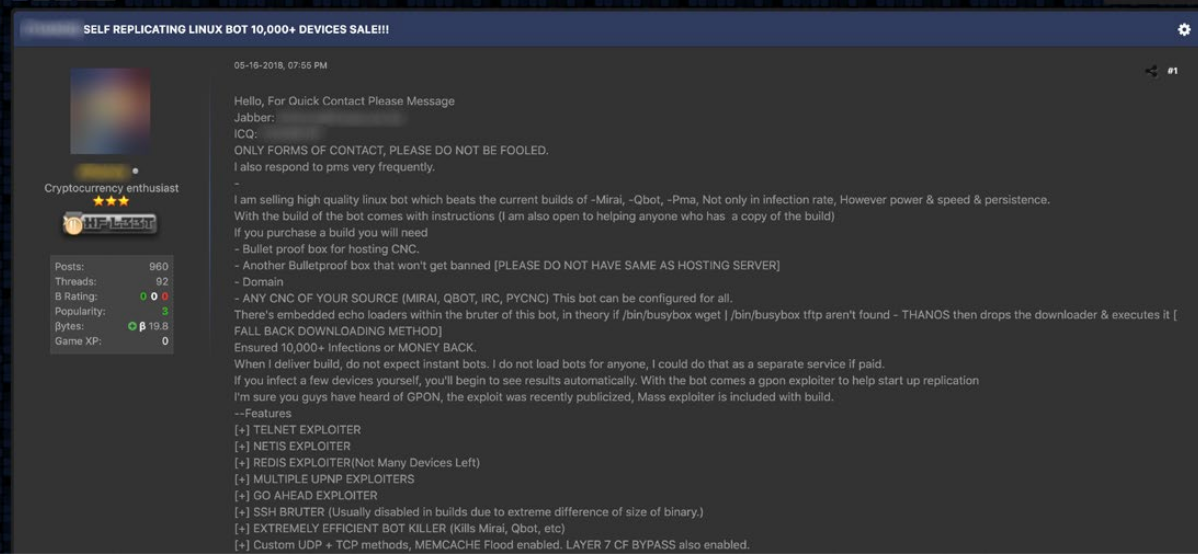
\includegraphics[width=0.8\textwidth]{figs/hf_sale_iot.png}
	\caption{IoT botnet for sale on Hack Forums}
	\label{fig:hf_sale_iot}
\end{figure}

\subsection{Forums}
\label{sec:forums}

First it is needed to identify most relevant underground forums. As stated by work done by Akyazi, U., van Eeten, M. J. G., \& Hernandez Ganan, C \cite{measuringCaaS}, based on \textit{CrimeBB} \cite{crimeBB} database from Cambridge Cybercrime Centre, most relevant underground forums (in order of relevance) are:

\vspace{0.5cm}

\begin{tabular}{llrrrr}
    \hline
    Forum & Language & Members & Threads & Posts & Oldest \\
    \hline
    Hackforums & EN & 573925 & 3856143 & 40196641 & 01/2007 \\
    Multiplayer Game Hacking & EN & 452186 & 739527 & 8907938 & 12/2005 \\
    Antichat & RU & 77865 & 242408 & 2449221 & 05/2002 \\
    RaidForums & EN & 43278 & 33100 & 124776 & 03/2015 \\
    Offensive Community & EN & 10593 & 18436 & 58779 & 06/2012 \\
    SafeSkyHacks & EN & 7378 & 12892 & 26842 & 03/2013 \\
    Kernelmode & EN & 1441 & 3144 & 25024 & 03/2010 \\
    Garage4Hackers & EN & 872 & 2096 & 7697 & 07/2010 \\
    Stresserforums & EN & 764 & 708 & 7069 & 04/2017 \\
    Greysee & EN & 440 & 1239 & 6969 & 06/2015 \\
    \hline
\end{tabular}
\\
\\
The information collected in crimeBB, with the activity of the underground forums, is a vast data set with millions of records. Given the impossibility of covering all that information in this work, it is decided to analyze the information contained in Hack Forums, as it is the largest.

\newpage
\chapter{Design and Development}
\label{chapter:designanddevelopment}

\section{Data source}

\subsection{CrimeBB}

Data source for current project is \textit{CrimeBB} \cite{crimeBB} database from Cambridge Cybercrime Centre. This database is made up of information collected from the main underground forums, through web scrapping. \\
Content of the database has been provided in the form of PostgreSQL dumps (.sql files). In order to make it possible to handle and query DB registries, these dump files have been loaded in a dockerized PostgreSQL database engine. \\
Steps needed for creating and Hydrating DB are described in project's source code \texttt{README.md} file. Files needed to do these steps are under \texttt{docker/postgres\_crimebb} folder.

\begin{figure}
	\centering
	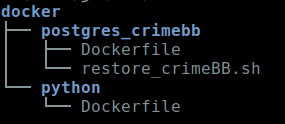
\includegraphics[width=0.4\textwidth]{figs/crimebb_tree.png}
	\caption{CrimeBB docker folder tree}
	\label{fig:crimebb_tree}
\end{figure}

\newpage

\subsection{Database structure}

Schema shown in image \ref{fig:crimebb_structure} describes how data models have been defined in it's tables, data field types and relations between them.

\begin{figure}[H]
	\centering
	\includegraphics[width=0.8\textwidth]{figs/crimebb.png}
	\caption{CrimeBB database structure}
	\label{fig:crimebb_structure}
\end{figure}

\noindent
\underline{NOTE}: \\
Schema shows relations between models, but provided DB data does not include foreign keys that ensure these relationships. That would be desirable in order to ensure data integrity.
\newpage

\section{Project Architecture}

\subsection{Overview}

All needed project components are self contained in a folder. It includes all needed \textit{Docker} and \textit{Docker-compose} stuff, \textit{Python} source code, generated datasets, \textit{Jupyter Workbook} ad so on ... \\
It is intended for allowing anyone to clone project's git repository and build up project in order to reproduce all results. For details on how to run it, see \texttt{README.md} in project root folder. \\
Just to prevent database content from being accidentally shared without permission, CrimeBB \texttt{.sql} dump files are not included in project folder. For the same reason, the container folder for the docker volume, from PostgreSQL, is also outside the project's root directory.

\subsection{Architecture}

Curent project source code architecture follows \textit{Hexagonal Architecture principles} (see figure \ref{fig:hexarch}), also known as \textit{Ports and Adapters}. This architecture was firstly described by Dr. Alistair Cockburn \cite{cockburn} and adopted by Steve Freeman, and Nat Pryce in their book \textit{Growing Object-Oriented Software Guided by Tests} \cite{growingoos}. \\
It is meant to be a flexible, changes ready way of structuring software projects. It is based in the \textit{Clean Code} principles, described by Robert C. Martin (Uncle Bob) in his well known \textit{The Clean Architecture} \cite{unclebob} article.
\newline
This architecture is divided in three main layers:
\begin{itemize}
    \item \textbf{Infrastructure}: The outer layer. Controllers and all I/O related stuff (DB access, file readers/writers, ...). Anything that can change by an "external" cause (not by your decision), is in this layer. It includes repositories specific implementation, known as \textit{adapters}. 
    \item \textbf{Application}: Use cases represented by application services. In essence, these are actions launched from outside, which aim to solve use cases typical of the business logic that this project intends to support.
    \item \textbf{Domain}: Inner layer. Business context and rules goes here, represented by models and domain services. Repository Interfaces, known as \textit{ports}, belongs to this layer.
\end{itemize}
\newpage

\begin{figure}[H]
	\centering
	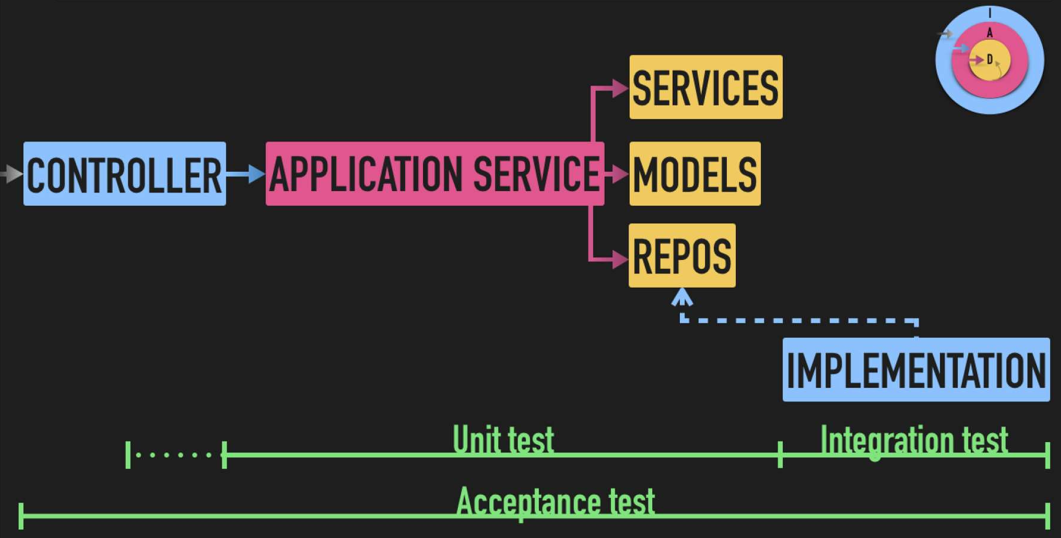
\includegraphics[width=0.8\textwidth]{figs/hex_arch_schema.png}
	\caption{Hexagonal Architecture}
	\label{fig:hexarch}
\end{figure}

This project has an important part of data exploration that makes it necessary to be able to change, in an agile way, the way to extract and process data. \\
Requirements could change along development process. According to that, main reasons for choosing this architecture are:
\begin{itemize}
    \item Layers distribution is intuitive. So it eases finding software component in the place that it is figured to be.
    \item Testing code is mandatory in order to build good quality software, reliable and easy to maintain. This architecture makes it easy to build software using \textit{TDD} (Test Driven Development) methodology.
    \item It allows to change the objectives, re-using as much code as possible, without the project structure ending up being a disaster.
\end{itemize}

\subsection{Testing}
In accordance with good practices widely accepted by the software developer community, Development has been done by following TDD (Test Driven Development) principles. TDD is now an established technique for delivering better software faster. TDD is based on a simple idea: writing tests for the code before writing the code itself. \\
For every layer, main component directories, contains a \texttt{tests/} folder with complete tests cases. Tests have been built with \texttt{unittest} Python library. \\
Running full tests battery is as easy as running the following command inside \texttt{python} docker container or within a Python virtual environment that meets \texttt{requirements.txt} packages:
\begin{verbatim}
    python -m unittest -v
\end{verbatim}

\section{Dataset generation helper software}
\label{sec:automaticprocess}

\textit{Ground truth} and \textit{full} datsets will contain \textit{HackForums} data. For this project, relevant data is placed in sub-forums under \textit{Market} section (the palce were services are supplied and demanded). \\
So, first step for building our datasets is to extract relevant data from Threads in these sub-forums. To do so, a Python tool has been built in order to connect to PostgreSQL DB and extract Threads and Posts from these subforums. \\
Once relevant information has been extracted from these Threads, DDoS related information is filtered and pre-annotated.

Resulting data is saved in a CSV dataset, that will be the seed of final datasets (see \autoref{sec:preannotate}). So, this pre-annotated datset,will be the starting point for the manual work necessary to prepare the \textit{supply} and \textit{demand} datasets that will be used to form the \textit{ground truth} and the \textit{full} datasets. \\
Both datasets, \textit{supply.csv} and \textit{demand.csv}, are the result of manual work. These datsets are then mixed and used for building \textit{ground truth} and \textit{full} (see \autoref{sec:builddatasets}). The former will be used for training and evaluating classification models and the latter is meant to be annotated by the selected model. That annotated full dataset will finally be used for data analysis in Jupyter Workbook.

\textbf{NOTE: } Manual work needed for creating \textit{supply.csv} and \textit{demand.csv} datasets is explained in \autoref{sec:datasetscreation}.

\newpage

\subsection{Generating pre-annotated dataset}
\label{sec:preannotate}

For generating pre-annotated dataset just execute Python tool entrypoint main file:
\begin{verbatim}
    python main.py annotate
\end{verbatim}
Resulting dataset CSV file is saved in project folder \texttt{datasets/ddos\_auto\_annotated\_dataset.csv} \\
The process can be summarized as shown in figure \ref{fig:preannotate}.

\begin{figure}[H]
	\centering
	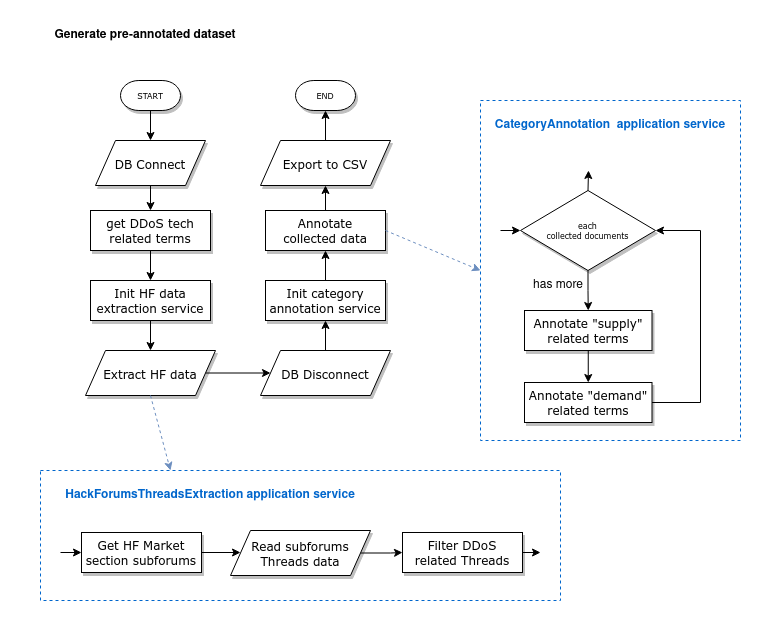
\includegraphics[width=1.0\textwidth]{figs/preannotate.png}
	\caption{Pre-annotate process}
	\label{fig:preannotate}
\end{figure}

\newpage

\subsection{Generating \textit{ground truth} and \textit{full} datasets}
\label{sec:builddatasets}

The result of manual work is \textit{supply.csv} and \textit{demand.csv} datasets. These datasets are then mixed to obtain \textit{ground truth} and \textit{full} datasets. To do that, Python tool is used as follows:
\begin{verbatim}
    python main.py generate_datasets
\end{verbatim}
In addition to the two above, two other datasets will be generated: \textit{market\_section\_posts\_count\_dataset.csv} and \textit{ddos\_posts\_count\_dataset.csv}. The former is a resume of HF market section posts count, grouped by month. The latter is the same but only DDoS related posts are included. These two datasets are intended to be used, later, in Jupyer Workbook. Process overview is shown in \ref{fig:generationprocess}

\begin{figure}[H]
	\centering
	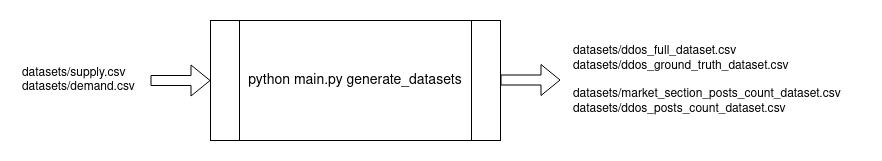
\includegraphics[width=0.8\textwidth]{figs/main.py.step2.png}
	\caption{Final datasets generation process}
	\label{fig:generationprocess}
\end{figure}

Figure \ref{fig:datasets_building} shows diagram flow on how all those four datasets are generated.

\begin{figure}[H]
	\centering
	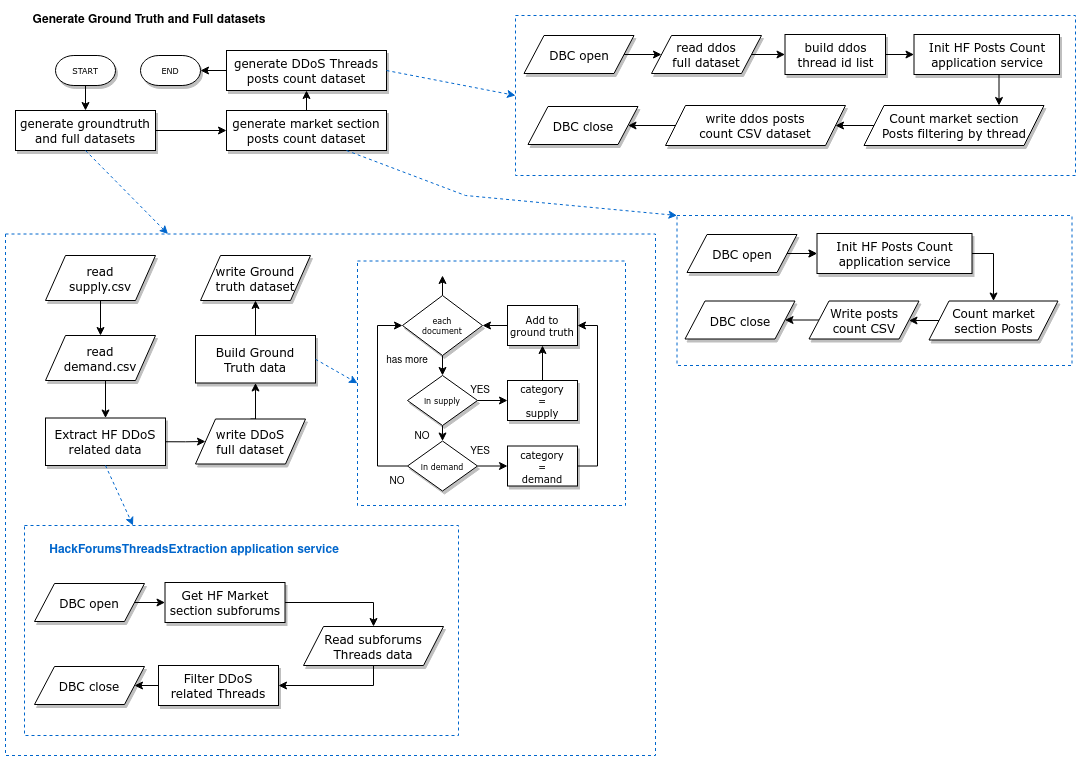
\includegraphics[width=1.0\textwidth]{figs/main.py_4_datasets.png}
	\caption{Final datasets generation detailed process}
	\label{fig:datasets_building}
\end{figure}

\section{Datasets creation process}
\label{sec:datasetscreation}

Datasets creation process consists in a mix of automated tasks and a lot of manual work. Automated processes have been covered in \autoref{sec:automaticprocess}. This section shows the full process.\\
Diagram \ref{fig:datasets_full_process} describes the workflow from when we generated the first pre-classified dataset, through manual refining and classification, to the construction of the final datasets.

\begin{figure}[H]
	\centering
	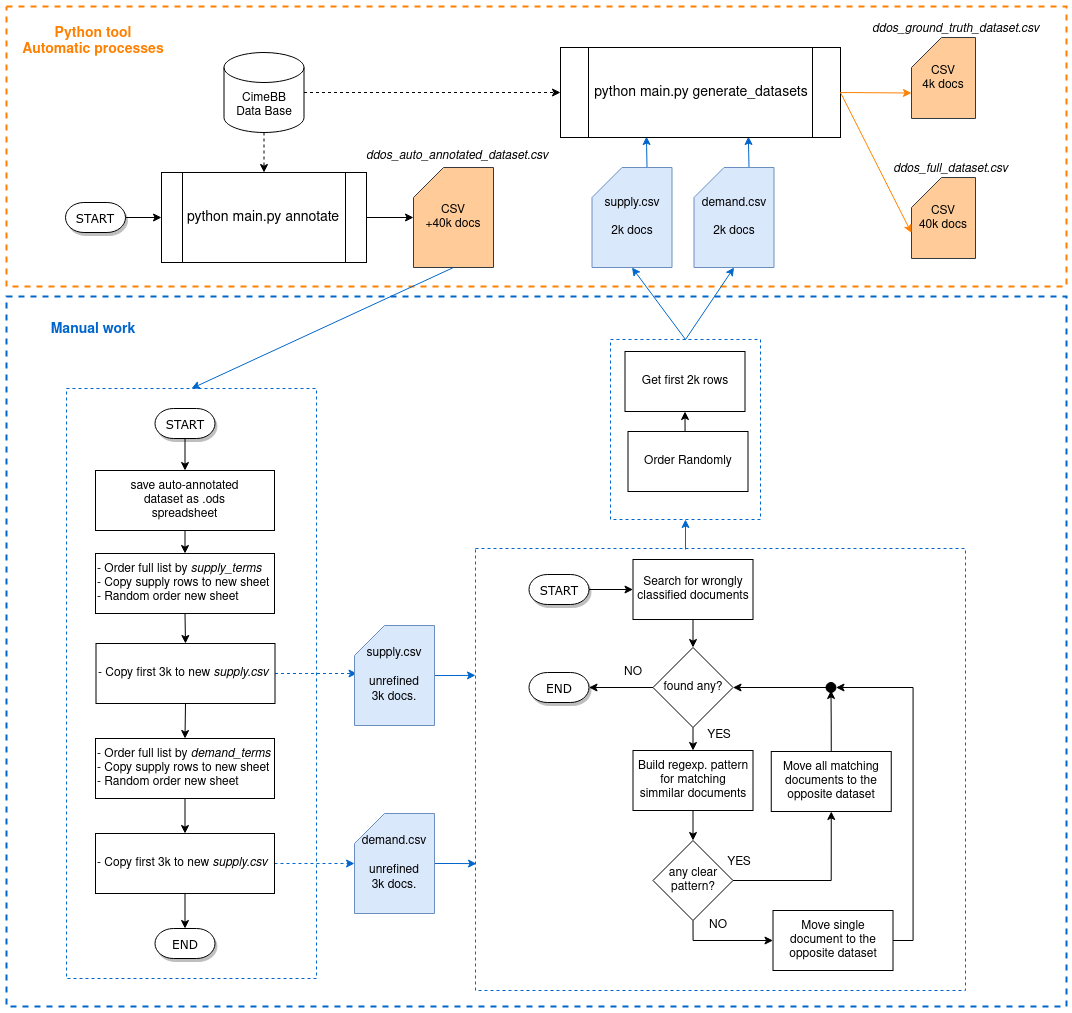
\includegraphics[width=1.0\textwidth]{figs/datasets_full_process.png}
	\caption{Final datasets generation detailed process}
	\label{fig:datasets_full_process}
\end{figure}

\section{Data analysis}
\label{sec:dataanalysis}

Final purpose of development phase is to analyse cimeBB DB data in order to know how \textit{Sale of access IoT devices} for DDoS is traded in underground forums.
Once annotated dataset and a full dataset have been built, data analysis tasks can be performed.\\
Jupyter Workbook has been selected as the tool for this final stage. It allows to write Python code and importing external libraries in order to load and analyse data and graph results. Despite data analysis and results obteined in Jupyter workbook are explained in chapter \ref{chapter:data_analysis_results}, this section describes main aspects of it.\\
Workbook sections are:
\begin{itemize}
    \item \textbf{Data source}: It loads datasets in pandas dataframes \cite{dataframe} and shows its structures.
    \item \textbf{Data pre-process}: Data clean, Tokenization and calculate \textit{tf and tf-idf} (Term Frequency times Inverse Document Frequency).
    \item \textbf{Model training}: Train some well known model types, commonly used in classification tasks (Linear Support Vector Classification, Stochastic Gradient Descent, K-nearest Neighbor, Multinomial Naïve Bayes).
    \item \textbf{Model evaluation}: Calculate \textit{accuracy}, \textit{precision}, \textit{recall} and \textit{F1 score}, and graph ROC curve in order to select best performing model.
    \item \textbf{Data Analysis}: In order to know how \textit{Sale of access IoT devices} has evolved in last years, we graph timeseries for main topics, segmenting by \textit{supply} and \textit{demand}. These main topics are: Supply \textit{vs} demand ratio, most used DD0S related tech terms, payment methods.
\end{itemize}

\newpage
\chapter{Data analysis and results}
\label{chapter:data_analysis_results}

\section{Data source}

Given all threads from Hack Forums Market section, each document is a mix of data: Thread heading and First post content and timestamp.\\
All threads from sub-forums in Market section have been pre-processed. Two datasets have been built by filtering all DDoS related threads:
\begin{itemize}
    \item \textit{ddos\_full\_dataset.csv}: ($>$40K docs, full dataset with all market section documents related with IoT DDoS.
    \item \textit{ddos\_groundtruth\_dataset.csv}: (4K docs), data sample. Randomly extracted from full dataset. Every doc category has been annotated by differenciating beteen \textit{supply} and \textit{demand}. This dataset is intended for training and testing text classification models.
\end{itemize}

All contents have been cleaned when building the datasets. Cleaning operations have been:
\begin{itemize}
    \item Lower case all text.
    \item Removed: punctuation, accents, non-textual content like citing, images, urls, ...
\end{itemize}

Ground truth dataset preview can be shown in figure \ref{fig:ground_truth_preview}.

\begin{figure}[H]
	\centering
	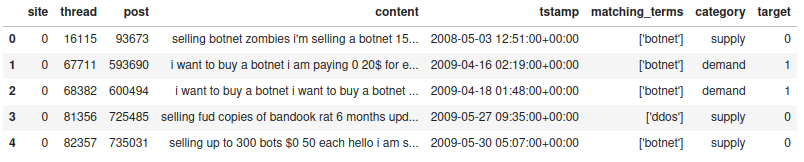
\includegraphics[width=1.0\textwidth]{figs/ground_truth_preview.png}
	\caption{Ground truth data preview}
	\label{fig:ground_truth_preview}
\end{figure}

Ground truth dataset has been split in two datasets for training and testing with 80/20 ratio. Resulting datasets have 3257 documents and 814 documents respectively.

\section{Data pre-process}

Since there are a lot of different words in corpus, result is a high dimensional dataset (too much different features). Building feature vectors with full word list is inefficient and can be unmanageable. This is why only non-zero parts of feature vectors are maintained in memory during analysis process. Main purpose of data pre-process phase is to reduce dataset dimensions. To do that, \textit{Tokenization} and \textit{Term Frequency calculations} techniques have been applied to dataset.

\subsection{Tokenization}

It consists in breaking down text in term vectors and filtering stop words. \textit{CountVectorizer} \cite{CountVectorizer} sklearn text feature extraction tool has been used for that purpose. It converts a collection of text documents (ground truth dataset \textit{content} column) to a matrix of token counts. This implementation produces a sparse representation of the counts.

\subsection{Term Frequency}

Some thread contents are longer than others, it can result in a higher average count values than shorter ones, but they really talk about same topic (category). Among that, some words appears in many documents in the corpus. These common words are less informative, so downscaling weights for these words is needed. In order to avoid this problem, a calculation tf and tf-idf (\textit{Term Frequency times Inverse Document Frequency}) has been done. Both (tf and tf-idf) are computed by TfidfTransformer \cite{TfidfTransformer}, a tool from sklearn text feature extraction.

\section{Model training}
\label{sec:training}

Accuracy has been tested for four well-known classification models. These models are widely used in classification tasks:
\begin{itemize}
    \item LinearSVC: Linear Support Vector Classification \cite{hsu2003practical}.
    \item SGD: Stochastic Gradient Descent \cite{ketkar2017stochastic}.
    \item K nearest Neighbors \cite{kozma2008k}.
    \item Multinomial Naïve Bayes \cite{kibriya2004multinomial}.
\end{itemize}

Performance metrics to be analysed are: precision, recall, F1-score and occurrences of each class (support). Confusion matrix will show, for each model, ratio of correct and wrong classification between categories (only two categories in our case).

\subsection{LinearSVC}
\label{sec:LinearSVC}

LinearSVC classification model accuracy has been 0.96. Figure \ref{fig:LinearSVC_cfm} shows its confusion matrix.
\begin{figure}[H]
	\centering
	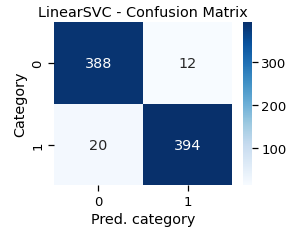
\includegraphics[width=0.3\textwidth]{figs/LinearSVC_cfm.png}
	\caption{LinearSVC confusion matrix}
	\label{fig:LinearSVC_cfm}
\end{figure}

\subsection{Stochastic Gradient Descent (SGD)}

Stochastic Gradient Descent classification model accuracy has been 0.93. Figure \ref{fig:sgd_cfm} shows its confusion matrix.
\begin{figure}[H]
	\centering
	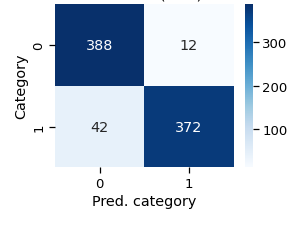
\includegraphics[width=0.3\textwidth]{figs/sgd_cfm.png}
	\caption{Stochastic Gradient Descent confusion matrix}
	\label{fig:sgd_cfm}
\end{figure}

\subsection{K-nearest neighbors}

K-nearest Neighbors classification model accuracy has been 0.79. Figure \ref{fig:knn_cfm} shows its confusion matrix.
\begin{figure}[H]
	\centering
	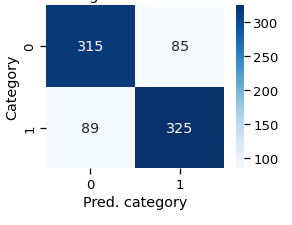
\includegraphics[width=0.3\textwidth]{figs/knn_cfm.png}
	\caption{K-nearest neighbors confusion matrix}
	\label{fig:knn_cfm}
\end{figure}

\subsection{Multinomial Naïve Bayes}

Multinomial Naïve Bayes classification model accuracy has been 0.89. Figure \ref{fig:mnb_cfm} shows its confusion matrix.
\begin{figure}[H]
	\centering
	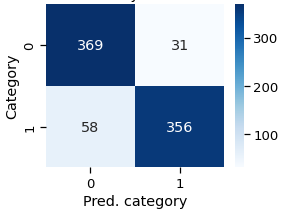
\includegraphics[width=0.3\textwidth]{figs/mnb_cfm.png}
	\caption{Multinomial Naïve Bayes confusion matrix}
	\label{fig:mnb_cfm}
\end{figure}

\section{Model evaluation}

\subsection{Metrics}

As stated in section \textit{Model training} \ref{sec:training}, performance metrics to be analysed are: precision, recall, F1-score and occurrences of each class (support). Results obtained in training stage are shown in figure \ref{fig:metrics}.

\begin{figure}[H]
	\centering
	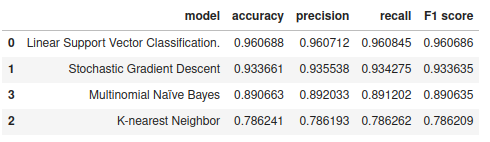
\includegraphics[width=0.7\textwidth]{figs/metrics.png}
	\caption{Training metrics report}
	\label{fig:metrics}
\end{figure}

\subsection{ROC curve}

The receiver operating characteristic (ROC) curve \cite{gonccalves2014roc} is frequently used for evaluating the performance of binary classification algorithms. It provides a graphical representation of a classifier’s performance, rather than a single value like most other metrics.

\begin{figure}[H]
	\centering
	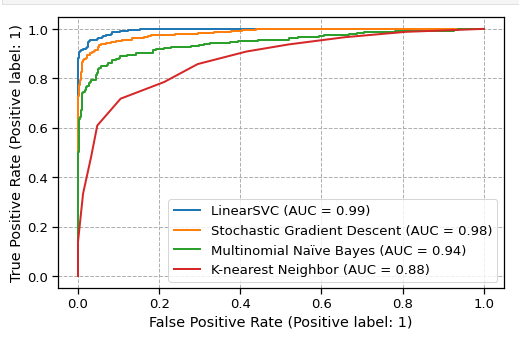
\includegraphics[width=0.7\textwidth]{figs/roc.png}
	\caption{ROC curve}
	\label{fig:roc}
\end{figure}

\subsection{Model selection}

According to evaluation results, best performing model is LinearSVC (Linear Support Vector Classifier) \ref{sec:LinearSVC}. Area under the curve in ROC curve figure \ref{fig:roc} and training metric values are close but better than Stochastic Gradient Descent model. The rest of the models clearly have worse results.

\section{Data Analysis}
\label{sec:analysis}

After selecting a prediction model, full dataset has been loaded and its documents have been labelled according to selected model prediciton results. An example on how documents have been labeled can is shown in figure \ref{fig:labels}

\begin{figure}[H]
	\centering
	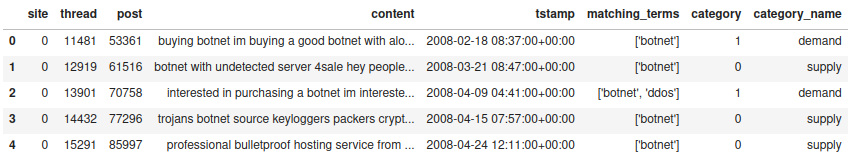
\includegraphics[width=1.0\textwidth]{figs/labels.png}
	\caption{Labeled documents example}
	\label{fig:labels}
\end{figure}

\subsection{Supply vs Demand}

Analysing evolution of supply and demand over time  allows to know how community members interest in that type of services have evolved of underground. It is the first step in analysing relevance of Sale of IoT devices for DDoS services in underground forums.

\begin{figure}[H]
	\centering
	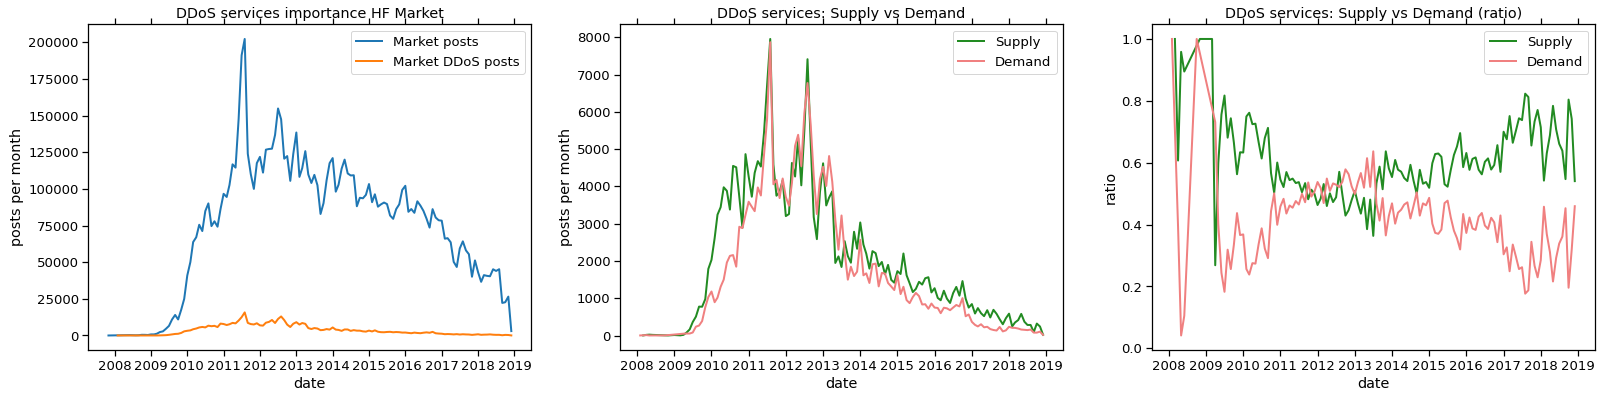
\includegraphics[width=1.0\textwidth]{figs/supply_vs_demand_full.png}
	\caption{Supply vs Demand posts volume in HF market}
	\label{fig:supply_vs_demand_full}
\end{figure}

As shown in fig. \ref{fig:supply_vs_demand_full}, supply did pass demand in 2012 and nowadays is clearly higher. However, according to results shown in fig. \ref{fig:terms} depending on the intention of the service, the demand may be higher than the supply. \\
This is happening today with \textit{stresser} related services. \textit{Stressers} are DDoS systems controlled by a professional operator. They are used to test the resistance of network systems against DDoS attacks.

\subsection{Relevant tech terms}

It is common to refer to \textit{Sale of access IoT devices services for DDoS} by using different tech terms like booter, stresser, ddoser, and so on. The use of some terms or others, when referring to these services, varies depending on the technology used to develop them, the intended use or simply the slang of the moment.

\begin{figure}[H]
	\centering
	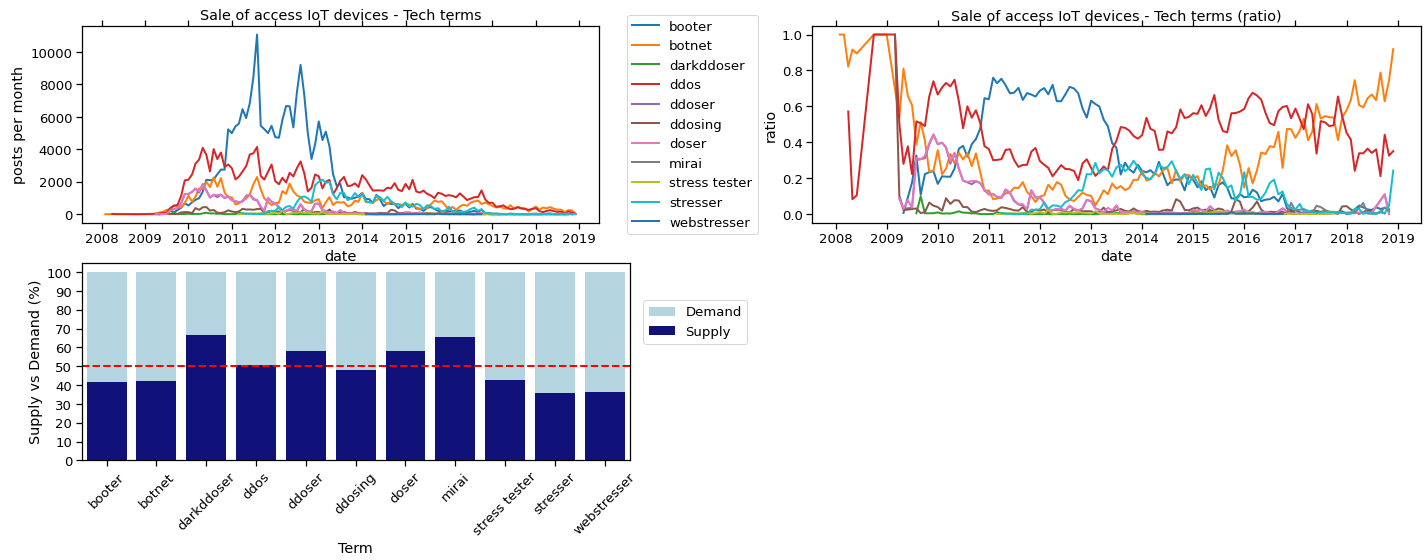
\includegraphics[width=1.0\textwidth]{figs/terms.png}
	\caption{Sale of access IoT devices - DDoS Tech terms}
	\label{fig:terms}
\end{figure}

\subsection{Preferred payment methods}

Fig. \ref{fig:payment_methods} shows how preferred payment methods, used for the Sale of access IoT devices, have evolved in last years. It is a key point in order to understand economics behind that type of criminal services.

\begin{figure}[H]
	\centering
	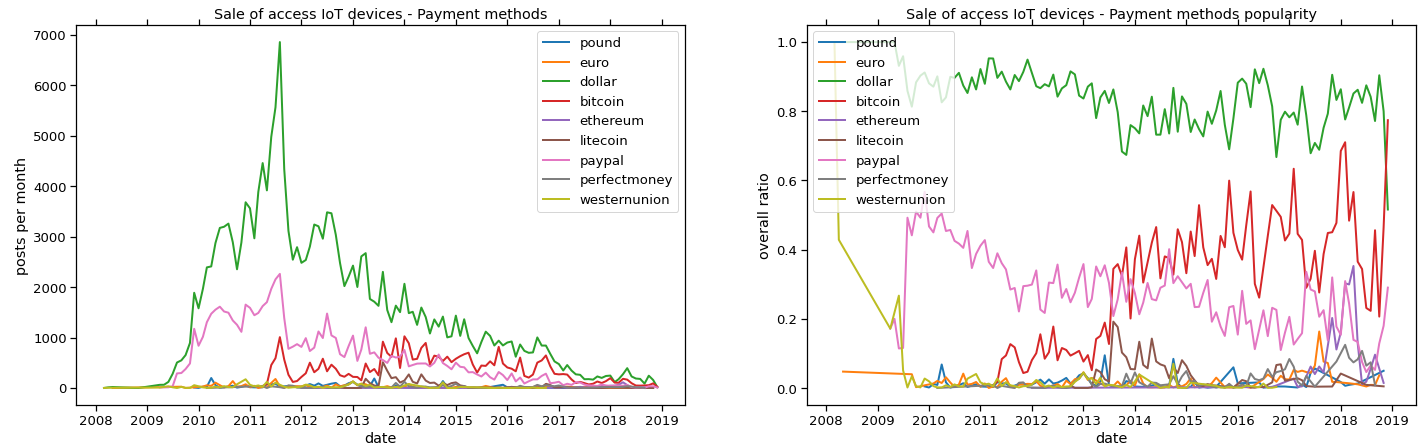
\includegraphics[width=1.0\textwidth]{figs/payment_methods.png}
	\caption{Preferred payment methods}
	\label{fig:payment_methods}
\end{figure}

The use of bitcoin as a preferred payment method has grown strongly in recent years. 
\newpage
\chapter{Conclusions}
\label{chapter:conclusions}

Data obtained in \textit{Data Analysis} section \ref{sec:analysis} reveals that underground forums as HackForums are clearly lossing market activity over last years. Sale of access IoT devices services for DDoS has been a very important topic in the market section, but the current trend is downward and it is no longer a topic of great relevance. 

However, the data obtained in this study do not allow us to affirm that the sale of this type of services has lost importance. Other forms of communication such as Telegram or Discord channels or other social networks could be gaining users to the detriment of this type of web forums. It could be due to its higher level of anonymity, ease of use and instant messaging benefits.

Regarding supply and demand, it seems that the interest of potential buyers has been declining and there is more activity in the supply than interest in buying. Although as an exception, it seems that services with a stress-as-a-service approach currently continue to have more demand than supply. Which suggests that there is a niche of professional buyers interested in hiring criminal services in order to test the resilience of their network systems.

Preferred payment methods have evolved significantly. The use of cryptocurrencies, more specifically Bitcoin, as a preferred payment method has been growing, being clearly more used nowadays. As we discussed earlier regarding forms of communication, the adoption of cryptocurrencies could be due to their higher level of anonymity, ease of use, and availability around the world. 
\newpage
\chapter{Future work}
\label{chapter:future}

AS stated in \ref{sec:forums} section, underground forums activity collected in crimeBB database is a vast amount of information. A possible future line of work is to analyze the information contained in the rest of the underground forums and analyze the results by comparing them.

In the present study it has not been possible to analyze the evolution of prices regarding sale of access IoT devices services for DDoS.  Analising price evolution in last years could be an interesting line of future work.

\newpage
\chapter{Source code}
\label{chapter:source}

Source code developed for current study is available, under \href{https://www.gnu.org/licenses/gpl-3.0.html}{GNU General Public License v3.0}, in author's public Github repository:\\
\href{https://github.com/serfer2/tfm}{https://github.com/serfer2/tfm}
\\
\\
The purpose of this repository is to allow any interested person to reproduce the results obtained.\\
Source code is divided in four main areas:

\begin{itemize}
    \item Infrastructure: It includes all resources needed in order to port and deploy project infrastructure, over docker containers, and for hydrating database.
    \item Data extraction and preprocess: It is Python helper software meant to assist in datasets creation.
    \item Data analysis: Jupyter Workbook used for models trainning, data analysis and building graphs.
    \item Documentation: LaTeX sources for current doc.
\end{itemize}




% bibliografia
\addcontentsline{toc}{chapter}{Bibliography}
\bibliographystyle{plain}
\bibliography{references}

\end{document}